\documentclass[12pt]{article}  % standard LaTeX, 12 point type
\usepackage{amsfonts,latexsym}
\usepackage{amsthm}
\usepackage{amssymb}
\usepackage[utf8x]{inputenc} % Кодировка
\usepackage[english]{babel} % Многоязычность
\usepackage{amsmath}
\usepackage{tikz}
\usetikzlibrary{automata,positioning}

\newtheorem{theorem}{Theorem}[section]
\newtheorem{proposition}[theorem]{Proposition}
\newtheorem{lemma}[theorem]{Lemma}
\newtheorem{corollary}[theorem]{Corollary}
\newtheorem{conjecture}[theorem]{Conjecture}

\theoremstyle{definition}
\newtheorem{definition}{Определение}[section]
\newtheorem{example}{Example}[section]

% unnumbered environments:

\theoremstyle{remark}
\newtheorem*{remark}{Remark}
\newtheorem*{notation}{Notation}
\newtheorem*{note}{Note}

\setlength{\parskip}{5pt plus 2pt minus 1pt}
%\setlength{\parindent}{0pt}

\usepackage{color}
\usepackage{listings}
\usepackage{caption}
\usepackage{graphicx}
\usepackage{ucs}

\newcommand{\tab}[1][0.3cm]{\ensuremath{\hspace*{#1}}}
% A generalized view on parsing and translation
% http://dl.acm.org/citation.cfm?id=2206331
\title{Brzozowski’s Derivatives for CFPQ}
% Context-free path querying ...
\author{Semyon Grigorev
\\
       {Saint Petersburg State University}\\
       {7/9 Universitetskaya nab.}\\
       {St. Petersburg, 199034, Russia}\\
       semen.grigorev@jetbrains.com, rsdpisuy@gmail.com
       }
\date{}

\begin{document}

\maketitle



Consider a context-free grammar $\mathcal{G}=(\Sigma, N, P, S)$ in BNF where $\Sigma$ is a terminal alphabet, $N$ is 
a nonterminal alphabet, $P$ is a set of productions, $S \in N$ is a start nonterminal.
Also we denote a directed labeled graph by $G=(V,E,L)$ where $E \subseteq V \times L \times V$ and $L \subseteq \Sigma$. 

We want to use Brzozowski’s derivatives for $\text{CFPQ}(\mathcal{G},G)$.
One of problems is a cycles and recursion interaction.
Possible solution is based on nonterminal naming: each nonterminal should has a form $_{u}N_{v}$ where $u\in V$ and $v \in V$. 
This meens that nonterminal with name $_{u}N_{v}$ corresponds to derivative computed along some (in final grammar --- along all) paths from $u$ to $v$.
If there are more than one path from $u$ to $v$, then there are more than one production for $_{u}N_{v}$.

Let the input graph is
\\
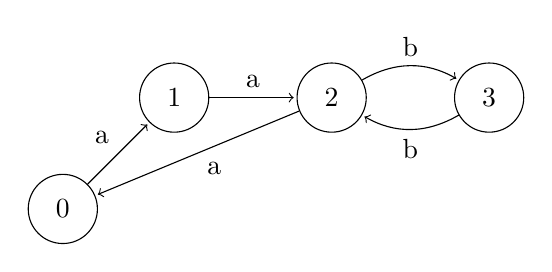
\begin{tikzpicture}[shorten >=1pt,node distance=2cm,on grid,auto] 
   \node[state] (q_0)   {$0$}; 
   \node[state] (q_1) [above right=of q_0] {$1$}; 
   \node[state] (q_2) [right=of q_1] {$2$}; 
   \node[state] (q_3) [right=of q_2] {$3$};
    \path[->] 
    (q_0) edge  node {a} (q_1)          
    (q_1) edge  node {a} (q_2)
    (q_2) edge  node {a} (q_0)
    (q_2) edge[bend left, above]  node {b} (q_3)
    (q_3) edge[bend left, below]  node {b} (q_2);
\end{tikzpicture}

 
Let the input grammar is 
\begin{align*}
S & \rightarrow a \ S \ b \ | \ a \ b 
\end{align*}

Let we try to compute derivative of this grammar from vertex 2.
This vertex in cycle and grammar has a recursion which should ``aggressively'' interact with this cycle: cycle produce sequence of arbitrary number of $a$ and any of these sequence may be a prefix of string produced by grammar.
In the example below we show that derivative computation may be done in finite number of steps.

\begin{enumerate}

\item Edge $2 \xrightarrow{a} 0$.

\begin{align*}
_{2}S_0 & \rightarrow S \ b \ | \ b 
\\
S & \rightarrow a \ S \ b \ | \ a \ b 
\end{align*}


\item Edge $0 \xrightarrow{a} 1$.

\begin{align*}
_{2}S_1 & \rightarrow \ _{0}S_1 \ b 
\\
_{0}S_1 & \rightarrow \ S \ b \ | \ b 
\\
S & \rightarrow \ a \ S \ b \ | \ a \ b 
\end{align*}


\item Edge $1 \xrightarrow{a} 2$.

\begin{align*}
_{2}S_2 & \rightarrow \ _{0}S_2 \ b  
\\
_{0}S_2 & \rightarrow \ _{1}S_2 \ b  
\\
_{1}S_2 & \rightarrow \ S \ b \ | \ b 
\\
S & \rightarrow \ a \ S \ b \ | \ a \ b 
\end{align*}

\item Edge $2 \xrightarrow{a} 0$.

\begin{align*}
_{2}S_0 & \rightarrow \ _{0}S_0 \ b  
\\
_{0}S_0 & \rightarrow \ _{1}S_0 \ b  
\\
_{1}S_0 & \rightarrow \ _{2}S_0 \ b  
\\
_{2}S_0 & \rightarrow \ S \ b \ | \ b 
\\
S & \rightarrow \ a \ S \ b \ | \ a \ b 
\end{align*}

\item Edge $0 \xrightarrow{a} 1$.

\begin{align*}
_{2}S_1 & \rightarrow \ _{0}S_1 \ b  
\\
_{0}S_1 & \rightarrow \ _{1}S_1 \ b  
\\
_{1}S_1 & \rightarrow \ _{2}S_1 \ b  
\\
_{0}S_1 & \rightarrow \ S \ b \ | \ b 
\\
S & \rightarrow \ a \ S \ b \ | \ a \ b 
\end{align*}


\item Edge $1 \xrightarrow{a} 2$.

\begin{align*}
_{2}S_2 & \rightarrow \ _{0}S_2 \ b  
\\
_{0}S_2 & \rightarrow \ _{1}S_2 \ b  
\\
_{1}S_2 & \rightarrow \ _{2}S_2 \ b  
\\
_{1}S_2 & \rightarrow \ S \ b \ | \ b 
\\
S & \rightarrow \ a \ S \ b \ | \ a \ b 
\end{align*}


\item Edge $2 \xrightarrow{a} 0$.

\begin{align*}
_{2}S_0 & \rightarrow \ _{0}S_0 \ b  
\\
_{0}S_0 & \rightarrow \ _{1}S_0 \ b  
\\
_{1}S_0 & \rightarrow \ _{2}S_0 \ b  
\\
_{2}S_0 & \rightarrow \ S \ b \ | \ b 
\\
S & \rightarrow \ a \ S \ b \ | \ a \ b 
\end{align*}


Given grammar is equal to grammar from step 4, so we can stop computations.


\end{enumerate}


When grammar is in the presented form, then nonterminal with name $_{u}N_{v}$ is nullable iff there is a path form $u$ to $v$ derivable from $N$.

Open problems.
\begin{itemize}
\item How grammar should be presented for efficient derivatives computation and efficient comparison?
\item How can we efficiently handle recomputations?
For example in case when we add new production for any previously existing nonterminal.
This question is related with data transferring in BSP model: we should propose some mechanism which can avoid unnecessary recomputations in BSP environment.
\end{itemize}


Seems that main idea from~\cite{DerForReg} can be reused ``as is''.
Vertices should exchange messages which contain derivative, check nullability and compute derivatives for outgoing edges if they were not computed in previous steps.
It is possible to prove that process is finite: $V$ and $N$ are finite sets, so a total number of new nonterminals is finite.
Proof of correctness looks challenging.


\begin{thebibliography}{9}



\bibitem{DerForReg}
Maurizio Nolé and Carlo Sartiani. 2016. Regular Path Queries on Massive Graphs. In Proceedings of the 28th International Conference on Scientific and Statistical Database Management (SSDBM '16), Peter Baumann, Ioana Manolescu-Goujot, Luca Trani, Yannis Ioannidis, Gergely Gábor Barnaföldi, László Dobos, and Evelin Bányai (Eds.). ACM, New York, NY, USA, Article 13, 12 pages. DOI: https://doi.org/10.1145/2949689.2949711



\end{thebibliography}


\end{document}